\documentclass[conference]{IEEEtran}
\IEEEoverridecommandlockouts
% The preceding line is only needed to identify funding in the first footnote. If that is unneeded, please comment it out.
%Template version as of 6/27/2024

\usepackage{cite}
\usepackage{amsmath,amssymb,amsfonts}
\usepackage{algorithmic}
\usepackage{graphicx}
\usepackage{textcomp}
\usepackage{xcolor}
\usepackage{svg}
\def\BibTeX{{\rm B\kern-.05em{\sc i\kern-.025em b}\kern-.08em
    T\kern-.1667em\lower.7ex\hbox{E}\kern-.125emX}}
\begin{document}

\title{Rich Communication Services\\als Nachfolger der SMS}

\author{\IEEEauthorblockN{David Olbertz}
    \IEEEauthorblockA{\textit{Hochschule Bonn-Rhein-Sieg} \\
        Sankt-Augustin, Germany \\
        davidolbertz@gmail.com}
}

\maketitle

\begin{abstract}
    Der Abstract wurde noch nicht verfasst.
\end{abstract}

\begin{IEEEkeywords}
    Diese, index, terms, existieren, noch, nicht
\end{IEEEkeywords}

\section{Einleitung}
Heutzutage ist das Smartphone ein wichtiger Bestandteil des Alltags.
Es ermöglicht unter anderem die Kommunikation über große Distanzen hinweg, egal ob im privaten oder beruflichen Umfeld.

Zur Kommunikation existiert neben der Telefonie der altbekannte Short Message Service (SMS), welcher es ermöglicht, einfache Kurznachrichten zu versenden.
Allerdings wird diese Kommunikationsmethode mittlerweile immer weniger genutzt und wurde größtenteils durch Over-the-Top Instant Messenger, welche deutlich mehr Funktionalitäten bieten, wie z.B. Gruppenchats und das Teilen von Medien.
Zusätzlich sind Nachrichten meist Ende-zu-Ende-Verschlüsselt und das Senden ist gebührenfrei \cite{ottmobinter}.
Dieser Trend bewegte die GSM Association dazu, einen neuen moderneren Kommunikationsstandard zu entwickeln, welcher ähnliche Funktionen wie die Over-the-Top Instant Messenger bieten.
Anders ist, dass es von Mobilfunkbetreibern anstatt von einem großen Unternehmen betrieben wird und dadurch auf fast allen Endgeräten verfügbar ist \cite{uniprof,rcsmno}.

Ziel dieser Seminararbeit ist, Rich Communication Services (RCS) als Nachfolger der SMS zu betrachten.
Dazu werden zuerst die aktuell gängigen Technologien behandelt und anschließend auf RCS im Detail eingegangen.
Neben der Definition und Funktionsweise werden auch weitere Aspekte, wie die Vor- und Nachteile der RCS, dargestellt.
Dabei werden auch die Eigenschaften von RCS mit denen von SMS verglichen, wobei besonders in heutigen Zeiten die Sicherheit eine große Rolle spielt.

\section{Entwicklung}

\subsection{Short Message Service}

Der Short Message Service, kurz SMS, ist seit den späten 1990er Jahren im Einsatz \cite{sendoutsms}.
Dafür wurde der Global System for Mobile Communications Standard etabliert, welcher von dem European Telecommunications Standards Institute entwickelt wurde \cite{smshow}.
SMS erlaubt es Nutzern mittels eines Mobiltelefons kurze Textnachrichten an andere Personen zu verschicken, unabhängig von der Distanz \cite{sendoutsms}.
Die Nachrichten können standardmäßig in der 7-Bit-Kodierung eine Länge von 160 Zeichen haben.
Das SMS Protokoll besteht aus 4 Schichten, die alle Informationen zum Versenden, wie unter anderem den Empfänger und der Nachrichteninhalt selbst, enthalten.
Zu den Schichten gehört der Application Layer, Transfer Layer, Relay Layer und Link Layer \cite{smshow}.

Damit Nachrichten überhaupt über große Distanzen versendet und empfangen werden können, wird eine gewisse Infrastruktur für den Mobilfunk benötigt.
Das Mobilfunknetz besteht aus Basisstationen, mit denen sich die Endgeräte drahtlos verbinden können, und aus Short Message Service Centers (SMSC), welche die versendeten Nachrichten an den korrekten Empfänger weiterleiten \cite{sendoutsms}.
Falls der Empfänger aus irgendeinem Grund nicht erreichbar ist und die Nachricht nicht zugestellt werden kann, wird sie im SMSC temporär gespeichert. Sobald der Empfänger wieder erreichbar ist, wird die Nachricht endgültig zugestellt und aus dem SMSC gelöscht \cite{smshow}.
Während der Übermittlung der Nachricht ist der Bereich zwischen dem Endgerät und der Basisstation verschlüsselt, innerhalb des Mobilfunknetzes allerdings nicht mehr \cite{sendoutsms}.

\begin{figure}[htbp]
    \centerline{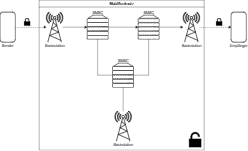
\includegraphics{mobilfunknetz.png}}
    \caption{Beispiel Mobilfunknetz}
\end{figure}

External Short Message Entities (ESME) sind ebenfalls Bestandteil des Netzes und werden meist von Unternehmen genutzt.
Verwendungszweck dafür ist das Senden und Empfangen einer großen Menge an Nachrichten.
Dies wird z.B. für das Versenden von One-Time-Passwords oder Notfallmeldungen genutzt.
ESMEs fungieren also als Schnittstelle und erlauben so einen direkten Zugriff auf die SMSCs oder Verkaufen den Zugriff an Dritte weiter.
Es existieren zum Beispiel Systeme, die einzelne Telefonnummern auf einer Website öffentlich zugänglich machen, damit Nutzer ohne Angabe persönlicher Daten darüber Nachrichten empfangenen kann.
Das wird teilweise noch weiter getrieben, sodass es Dienste gibt, bei denen man ganz einfach an Telefonnummern kommt, mit denen auch Nachrichten versendet werden können.
Da hier wieder keine Angaben persönlicher Daten notwendig sind, werden solche Nummern oft für Betrugszwecke ausgenutzt.
Nicht zuletzt sollte aus Sicht des Datenschutzes beachtet werden, dass die gesendeten und empfangenen Nachrichten eventuell für längere Zeit von ESMEs gespeichert werden \cite{sendoutsms}.


\subsection{Over-the-Top Instant Messenger}

\begin{itemize}
    \item jeder Nutzer muss Client installieren
\end{itemize}
\cite{rcsmno}

\dots

Ein populäres Beispiel für einen OTT Messenger ist WhatsApp.
WhatsApp wurde ursprünglich 2009 als eigenständiges Unternehmen gegründet und ist seit 2014 Teil von Meta Platforms Inc \cite{watimeline}.
Früher war die Nutzung des Dienstes mit einem kostenpflichtigen Abo verbunden, ist allerdings mittlerweile vollständig kostenlos nutzbar \cite{wakostenlos}.

Der WhatsApp Messenger bietet zahlreiche Funktionen an, die über einfache Textnachrichten hinaus gehen.
Es ist möglich, verschiedene Arten von Medien zu versenden, wie unter anderem Fotos, Videos, Audio und Dokumente.
Weitere Nachrichtentypen, wie Live-Standort und Kontaktdaten sind ebenfalls vorhanden.
Auf Nachrichten kann mit Emojis reagiert werden.
Für sensiblere Nachrichten gibt es die Möglichkeit, selbstlöschende Nachrichten zu aktivieren, welche nach einer voreingestellten Zeit oder nach einmaligem anschauen automatisch gelöscht werden \cite{wafaq}.
Damit die Sicherheit und Privatsphäre der Nutzer gewährleistet sind, sind alle Nachrichten Ende-zu-Ende-Verschlüsselt und können nur auf den entsprechenden Endgeräten der Nutzer entschlüsselt werden.
Der komplette Nachrichtenverkehr wird über die WhatsApp-Server abgewickelt \cite{waencryption}.
Gruppenchats erlauben die Kommunikation mit mehreren Personen gleichzeitig. Die Telefonie-Funktion beinhaltet den Videoanruf, welcher Live-Videos von den teilnehmenden Personen übertragen. Während dem Anruf kann man weiterhin auf die Chats zurückgehen und wie gewohnt parallel nutzen \cite{wafaq}.
Wer WhatsApp gerade nicht auf einem mobilen Endgerät nutzen möchte, kann auf WhatsApp Web oder WhatsApp Desktop ausweichen, um den Dienst auch auf anderen Plattformen wie Desktop-PCs zu nutzen.
Die Verknüpfung des Accounts findet über das Scannen eines QR-Codes statt \cite{wafaq,waencryption}.

Mit WhatsApp Business ist es möglich, dass Nutzer mit Unternehmen kommunizieren können. Dies kann für z.B. Support, aber auch automatisierte Chatbots genutzt werden. Allerdings muss bedacht werden, dass nicht alle Unternehmen direkt über WhatsApp Business kommunizieren, sondern mittels eines Dienstes Dritter über die WhatsApp API. Dadurch ist die Ende-zu-Ende-Verschlüsselung nicht mehr vollständig gewährleistet \cite{waencryption}.


\section{Rich Communication Services}

\subsection{Definition}

Seit dem Aufstieg von OTT sinkt die Nutzung von klassischen Kommunikationsarten wie SMS.
Laut einer Statistik der Bundesnetzagentur ist die Nutzung von SMS im Jahr 2015 bereits um 41 \% gesunken \cite{ottmobinter}.
2008 veröffentlichte die "Groupe Speciale Mobile Association" (GSMA) die erste Version des Universal Profiles, welche die Funktionen der Rich Communication Services (RCS) definiert \cite{rcsuite}.
Zu den Grundideen gehört unter anderem die Verknüpfung verschiedener Dienste, wie das Nachrichtenschreiben, die Kontakte-App und die Kontakte-App.
Außerdem sollen die Funktionen nativ im Betriebssystem implementiert sein.
Für die Implementierung sind die Entwickler des Betriebssystems bzw. der Gerätehersteller zuständig.
Beispiel dafür ist die Android-Implementierung in Google Messages \cite{googlemessages}.
Seit 2024 ist RCS auch auf iOS-Geräten über iMessage verfügbar \cite{applemessages}.
Alternativ gibt es die Möglichkeit, RCS-Funktionalität durch das Installieren einer dafür entwickelten App zu erhalten \cite{uniprof}.

\subsection{Funktionen}

\begin{itemize}
    \item Spam kann vermieden werden
\end{itemize}
\cite{uniprof}

Die Funktionen sind grundsätzlich in drei Kategorien eingeteilt: "Enriched Messaging", "Enriched Calling" und "Enriched Phonebook".
Beim "Enriched Messaging" gibt es das klassische "1-to-1 Messaging", sprich den Nachrichtenaustausch zwischen zwei Personen, wie man es auch von SMS kennt, und die Möglichkeit, in Gruppenchats mit mehreren Personen gleichzeitig zu kommunizieren.
Innerhalb der Chats ist es möglich, Dateien zu versenden.
Dabei kann jeder Dateityp versendet werden. Bestimmte Dateiformate werden auf eine bestimmte Weise im Chat dargestellt, wie z.B. pdf-Dateien mit Dokumentenvorschau, direkt im Chat abspielbare Audio-Dateien und animierte GIFs.
Bilder und Videos sind ebenfalls möglich.
Nach dem Senden kann für gesendete Dateien der Sende-Status eingesehen werden.
Dadurch kann geprüft werden, ob eine Datei korrekt versendet wurde oder ob der Transfer noch aussteht oder sogar fehlgeschlagen ist.
Sprachnachrichten können direkt in der App aufgenommen und verschickt werden.
Der aktuelle Standort des Senders kann ebenfalls geteilt werden, entweder als Snapshot oder Live-Standort.
Bei jeder verschickten Nachricht kann der Sender sehen, ob die Nachricht angekommen ist und ob sie bereits vom Empfänger gelesen wurde.
Außerdem sieht der Chatteilnehmer, wenn der jeweils Andere eine Nachricht am Eintippen ist.
Mit "Enriched Calling" kann man während einem Anruf unter anderem einen Dateitransfer durchführen.
Dies ermöglicht Videoanrufe, bei denen die Teilnehmer live die Aufnahme ihrer Kamera teilen können.

\cite{uniprof}

\dots

Die Idee beim "Enriched Phonebook" ist, dass Nutzer sich ihr eigenes Profil einrichten können.
Dadurch kann jeder andere Nutzer das Profil sehen.
(freiwillig, beide müssen Profil teilen)

\cite{rcsuite}

\dots

Anstatt nur mit Personen zu interagieren, existiert die Möglichkeit, mit Diensten zu kommunizieren. Dazu gehören Chatbots, wie z.B. die Integrierung von Gemini in Google Messages \cite{geminiinteg}, oder Chats zum Empfangen von 2FA-Codes. Diese Unternehmenskontakte beinhalten in deren Profil zusätzlich Informationen zum Chatbot bzw. zum Unternehmen.

\cite{uniprof}


\subsection{Technik}

Damit möglichst alle Funktionen von RCS reibungslos funktionieren, müssen sich die Mobilfunk-Operatoren auf eine gängige Implementierung einigen.
Um dies zu erreichen haben sich 2011 mehrere große Unternehmen, darunter die Deutsche Telekom, Telefonica und Vodafone angekündigt, einen Zusammenschluss zu bilden und eine gemeinsame RCS-Implementierung, auch RCS-e (Rich Communication Services enhanced) genannt, zu definieren \cite{rcsmno}.

Da aber trotz solchen Maßnahmen immer noch Implementierungsverschiedenheiten existieren können, existiert die "Capability Discovery"-Funktion.
Sie dient dazu, den Clients zu zeigen, welche RCS-Funktionen verfügbar sind.
Damit eine Funktion verfügbar ist, muss sie bei beiden Clients implementiert sein bzw. vom Mobilfunkanbieter unterstützt werden.
Falls die Funktionen verfügbar sind, werden sie automatisch aktiviert.
Falls dies nicht der Fall sein sollte, wird dem Nutzer angeboten, seine Nachricht alternativ als SMS zu verschicken \cite{uniprof}.
Dabei entscheidet der "Unified Composer", ob die Nachricht als SMS oder MMS (bei Mediendateien) verschickt werden muss \cite{rcsuite}.


\subsection{Sicherheit}

Um sich bei RCS zu authentifizieren, gibt es je nach Plattform unterschiedliche Methoden.
Auf mobilen Endgeräten wird meist die SIM-basierte Authentifizierung genutzt, sprich eine Anmeldung über die Telefonnummer. Auf anderen Geräten ohne SIM Karte werden andere Möglichkeiten für die Anmeldung genutzt, wie z.B. der Login mit Nutzername und Passwort oder die Verknüpfung mit dem mobilen Endgerät über das Einscannen eines QR-Codes \cite{uniprof}.

\dots

Alle Nachrichten sind während der Übertragung durch gängige Protokolle, wie TLS und IPSec, verschlüsselt \cite{uniprof}.
Falls beide Nutzer Google Messages verwenden, sind die Nachrichten zusätzlich Ende-zu-Ende-Verschlüsselt.
Diese Funktion funktioniert allerdings auch nur in diesem Fall, da die GSMA keine offizielle Implementierung definiert hat.
Dadurch ist dies nicht plattformübergreifend verfügbar \cite{googlemessagessecure}.


\section{Vorteile von RCS gegenüber SMS}

\begin{itemize}
    \item anstatt für jeden Instant Messenger eigenen Client zu installieren, der Leistung braucht, universeller integrierter Messenger
    \item es ist möglich, RCS über ein Mobilgerät oder auch PC zu nutzen
\end{itemize}
\cite{rcsmno}

\begin{itemize}
    \item man kann clients auf mehreren Geräten nutzen
    \item bei Dual-SIM ist RCS mit beiden Karten gleichzeitig möglich
\end{itemize}
\cite{uniprof}

\section{Schwächen von RCS}

\begin{itemize}
    \item SMS SIM Swap Attack
          \begin{itemize}
              \item Angreifer gibt sich als das Opfer aus, um neue SIM-Karte zu erhalten oder eine Umleitung einzurichten
              \item kann Nachrichten abfangen, wie One-Time-Passwords
              \item durch RCS nicht gelöst, da es auch über die Telefonnummer läuft
          \end{itemize}
\end{itemize}
\cite{sendoutsms}

\begin{itemize}
    \item alle Mobilfunkanbieter müssen zusammenarbeiten, damit die Kommunikation auch über Ländergrenzen hinweg nahtlos funktionieren kann, es sollte eine standardisierte Implementation geben
    \item alle Hersteller von Mobilgeräten müssen RCS implementieren, damit die Verbreitung besser vorangetrieben wird
\end{itemize}
\cite{rcsmno}

\begin{itemize}
    \item Samsung Messages
    \item Google Messages
    \item iMessage (nur neuste iOS Version)
\end{itemize}

\section{Fazit}

\dots

\begin{thebibliography}{00}
    \bibitem{ottmobinter} N. Wellmann, "Are OTT messaging and mobile telecommunication an interrelated market? An empirical analysis", Telecommun. Policy, Bd. 43, Nr. 9, Oktober 2019, doi: 10.1016/j.telpol.2019.101831.
    \bibitem{rcsmno} M. Lin und J. Arenzana Arias, "Rich Communication Suite: The challenge and opportunity for MNOs", in 2011 15th International Conference on Intelligence in Next Generation Networks, Okt. 2011, S. 187–190. doi: 10.1109/ICIN.2011.6081071.
    \bibitem{uniprof} GSMA. "RCS Universal Profile Service Definition Document". Zugegriffen: 06.11.2024. [Online]. Verfügbar unter: https://www.gsma.com/solutions-and-impact/technologies/networks/wp-content/uploads/2019/10/RCC.71-v2.4.pdf
    \bibitem{sendoutsms} B. Reaves, N. Scaife, D. Tian, L. Blue, P. Traynor, und K. R. B. Butler, "Sending Out an SMS: Characterizing the Security of the SMS Ecosystem with Public Gateways", in 2016 IEEE Symposium on Security and Privacy (SP), Mai 2016, S. 339–356. doi: 10.1109/SP.2016.28.
    \bibitem{watimeline} "Danke für 10 Jahre", WhatsApp.com. Zugegriffen: 4. Dezember 2024. [Online]. Verfügbar unter: https://blog.whatsapp.com/thank-you-for-10-years
    \bibitem{wakostenlos} "WhatsApp kostenlos und nützlicher machen", WhatsApp.com. Zugegriffen: 4. Dezember 2024. [Online]. Verfügbar unter: https://blog.whatsapp.com/making-whats-app-free-and-more-useful
    \bibitem{wafaq} "WhatsApp-Hilfebereich". Zugegriffen: 4. Dezember 2024. [Online]. Verfügbar unter: https://faq.whatsapp.com/
    \bibitem{waencryption} WhatsApp. "WhatsApp Encryption Overview Technical White Paper". Zugegriffen: 4. Dezember 2024. [Online]. Verfügbar unter: https://faq.whatsapp.com/820124435853543\#nachrichtenaustausch-mit-unternehmen
    \bibitem{rcsuite} K. Henry, Q. Liu, und S. Pasquereau, "Rich Communication Suite", in 2009 13th International Conference on Intelligence in Next Generation Networks, Okt. 2009, S. 1–6. doi: 10.1109/ICIN.2009.5357089.
    \bibitem{googlemessages} ""RCS-Chats" in Google Messages aktivieren - Google Messages". Zugegriffen: 16. Dezember 2024. [Online]. Verfügbar unter: https://support.google.com/messages/answer/7189714?sjid=174292638
    24577998783-EU\&hl=de
    \bibitem{applemessages} "Was ist der Unterschied zwischen iMessage, RCS und SMS/MMS? - Apple Support (DE)", Apple Support. Zugegriffen: 16. Dezember 2024. [Online]. Verfügbar unter: https://support.apple.com/de-de/104972
    \bibitem{geminiinteg} "Gemini in Google Messages verwenden - Google Messages". Zugegriffen: 16. Dezember 2024. [Online]. Verfügbar unter: https://support.google.com/messages/answer/14599070?hl=de
    \bibitem{smshow} J. Brown, B. Shipman, und R. Vetter, "SMS: The Short Message Service", Computer, Bd. 40, Nr. 12, S. 106–110, Dez. 2007, doi: 10.1109/MC.2007.440.
    \bibitem{googlemessagessecure} "So schützen wir die Vertraulichkeit von RCS-Chats - Google Messages". Zugegriffen: 23. Dezember 2024. [Online]. Verfügbar unter: https://support.google.com/messages/answer/9592174?sjid=2530033474
    497695451-EU\&hl=de\#zippy=\%2Chow-we-protect-your-data\%2Cso-sch\%C3\%BCtzen-wir-ihre-daten
\end{thebibliography}

\end{document}